\documentclass[12pt,border=5pt]{standalone}
\usepackage[T1]{fontenc}
\usepackage{lmodern,amsmath,amssymb,bm,tikz}
\usetikzlibrary{arrows.meta,positioning,calc,shapes.geometric,fit,matrix}
\newcommand{\RR}{\mathbb R}
\newcommand{\norm}[1]{\left\lVert#1\right\rVert}
\DeclareMathOperator{\col}{col}
\DeclareMathOperator{\diag}{diag}
\definecolor{plantblue}{HTML}{247BA0}
\definecolor{plantteal}{HTML}{16856B}
\definecolor{plantorange}{HTML}{D97425}
\definecolor{plantpurple}{HTML}{7954A1}
\begin{document}
\begingroup\linespread{1}\selectfont
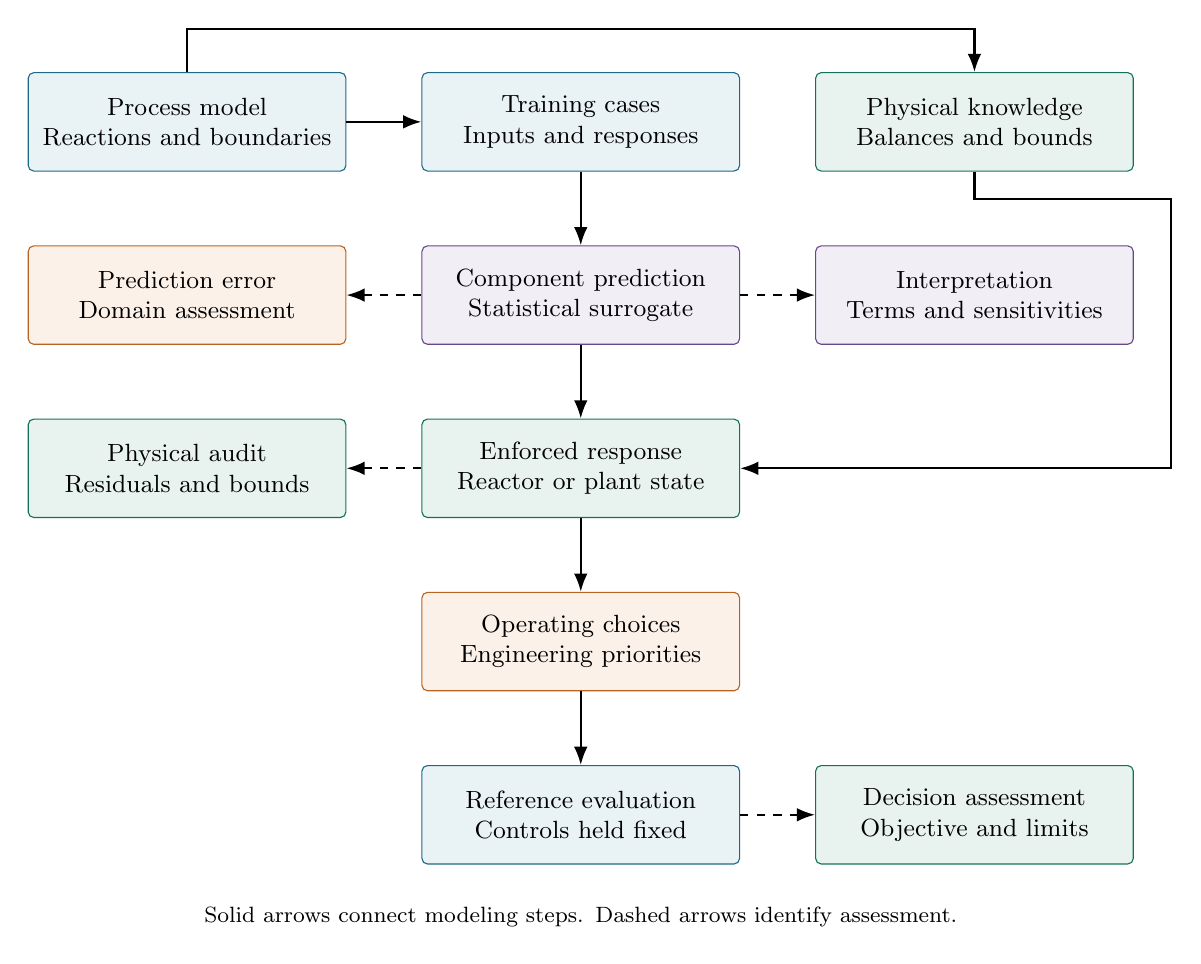
\begin{tikzpicture}[
  >=Latex,
  knowledge/.style={draw=plantblue!85!black,rounded corners=2pt,fill=plantblue!8,
    text width=3.8cm,minimum height=1.25cm,align=center,font=\small},
  stage/.style={draw=plantblue!85!black,rounded corners=2pt,fill=white,
    text width=3.8cm,minimum height=1.25cm,align=center,font=\small},
  evidence/.style={draw=plantblue!70!black,rounded corners=2pt,fill=plantteal!9,
    text width=3.8cm,minimum height=1.25cm,align=center,font=\small},
  construction/.style={->,thick},
  assessment/.style={->,dashed,thick}
]
\node[knowledge,draw=plantblue!85!black,fill=plantblue!10] (mechanism) at (0,0)
  {Process model\\Reactions and boundaries};
\node[knowledge,draw=plantblue!85!black,fill=plantblue!10] (data) at (5.0,0)
  {Training cases\\Inputs and responses};
\node[knowledge,draw=plantteal!85!black,fill=plantteal!10] (physics) at (10.0,0)
  {Physical knowledge\\Balances and bounds};
\node[stage,draw=plantpurple!85!black,fill=plantpurple!10] (prediction) at (5.0,-2.2)
  {Component prediction\\Statistical surrogate};
\node[evidence,draw=plantorange!85!black,fill=plantorange!10] (accuracy) at (0,-2.2)
  {Prediction error\\Domain assessment};
\node[evidence,draw=plantpurple!85!black,fill=plantpurple!10] (inspection) at (10.0,-2.2)
  {Interpretation\\Terms and sensitivities};
\node[stage,draw=plantteal!85!black,fill=plantteal!10] (enforced) at (5.0,-4.4)
  {Enforced response\\Reactor or plant state};
\node[evidence,draw=plantteal!85!black,fill=plantteal!10] (audit) at (0,-4.4)
  {Physical audit\\Residuals and bounds};
\node[stage,draw=plantorange!85!black,fill=plantorange!10] (choice) at (5.0,-6.6)
  {Operating choices\\Engineering priorities};
\node[stage,draw=plantblue!85!black,fill=plantblue!10] (reference) at (5.0,-8.8)
  {Reference evaluation\\Controls held fixed};
\node[evidence,draw=plantteal!85!black,fill=plantteal!10] (decision) at (10.0,-8.8)
  {Decision assessment\\Objective and limits};
\draw[construction] (mechanism)--(data);
\draw[construction] (mechanism.north)--++(0,0.55)-|(physics.north);
\draw[construction] (data)--(prediction);
\draw[construction] (prediction)--(enforced);
\draw[construction] (physics.south)--++(0,-0.35)--++(2.5,0)
  |- (enforced.east);
\draw[assessment] (prediction)--(accuracy);
\draw[assessment] (prediction)--(inspection);
\draw[assessment] (enforced)--(audit);
\draw[construction] (enforced)--(choice);
\draw[construction] (choice)--(reference);
\draw[assessment] (reference)--(decision);
\node[align=center,text width=13.5cm,font=\footnotesize] at (5,-10.1)
  {Solid arrows connect modeling steps. Dashed arrows identify assessment.};
\end{tikzpicture}
\endgroup

\end{document}
